\model{Screenshots}

\textit{Write the name of the operating system under each screenshot:}

\begin{center}
\begin{tabularx}{\textwidth}{cXcXc}

% source: https://play.google.com/store/apps/details?id=com.acr.screenshothd
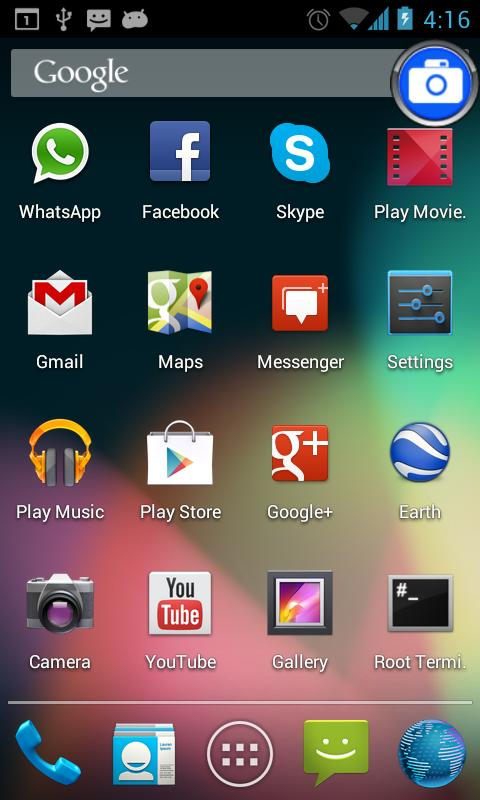
\includegraphics[height=93pt]{android.jpg}
&&
% source: http://www.omgchrome.com/simpler-app-launcher-lands-in-chromeos-dev/
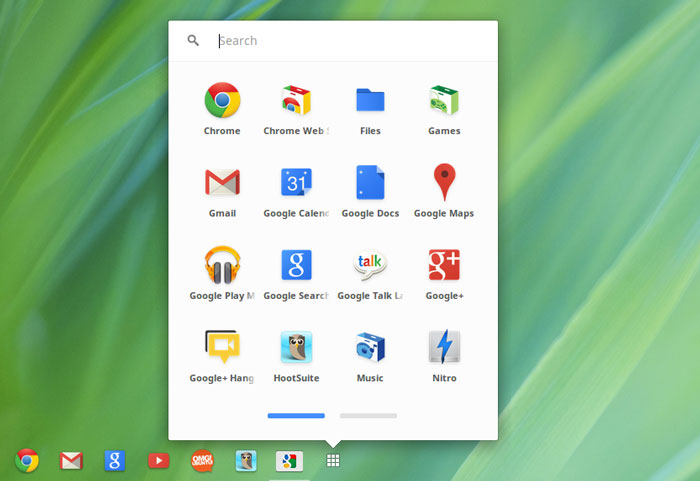
\includegraphics[height=93pt]{chrome.jpg}
&&
% source: http://www.cultofmac.com/230954/ios-7-in-action-gallery/
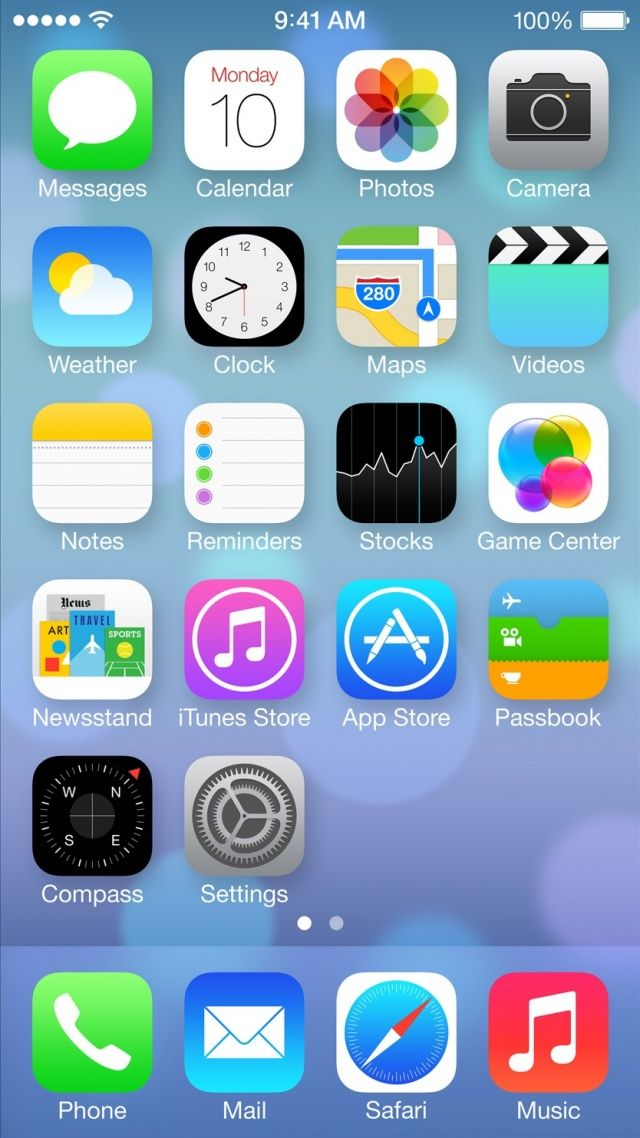
\includegraphics[height=93pt]{ios.jpg}

\\
\ans{Android}
&&
\ans{Chrome OS}
&&
\ans{iOS}
\vspace{1ex}

\\
% source: http://blog.linuxmint.com/?p=3026
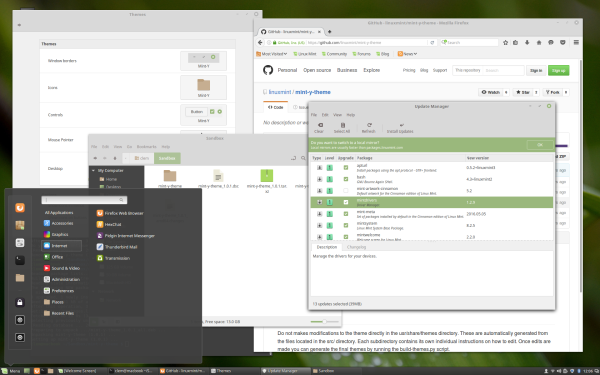
\includegraphics[height=93pt]{mint.png}
&&
% source: http://www.macworld.com/article/2987618/os-x/how-to-take-screenshots-on-your-mac.html
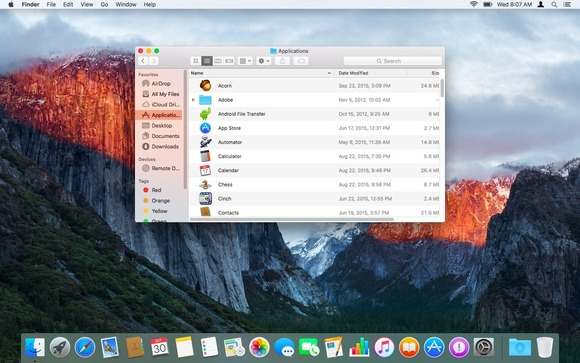
\includegraphics[height=93pt]{macos.jpg}
&&
% source: http://www.pcmag.com/article2/0,2817,2488631,00.asp
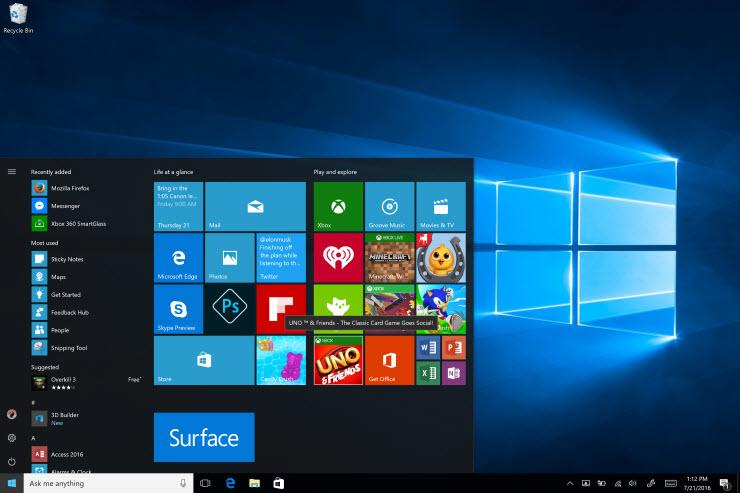
\includegraphics[height=93pt]{windows.jpg}

\\
\ans{Linux Mint}
&&
\ans{Mac OS}
&&
\ans{Windows}
\vspace{1ex}

\end{tabularx}
\end{center}


\quest{10 min}


\Q What do these operating systems have in common? Describe at least three similarities.

\begin{answer}
They each have a menu that allows the user to run applications by clicking on icons.
Users can run multiple applications at the same time (although it looks different).
All of these OS's have security updates that need to be applied on a regular basis.
\end{answer}


\Q How are these operating systems different? Describe at least three major differences.

\begin{answer}
They run on different types of hardware (phones, tablets, Chromebooks, desktops).
Different companies and organizations make them (Apple, Google, Microsoft, others).
They each have their own set of features, strengths, and weaknesses.
\end{answer}


\Q Based on your experience as a computer user, what does an operating system do?

\begin{answer}
The OS ``runs'' the computer: it manages the hardware, starts and stops applications, and provides the overall look and feel of the user experience.
\end{answer}
